\PassOptionsToPackage{hyphens}{url}
\documentclass[a4paper,twocolumn,11pt,unpublished]{quantumarticle}
\pdfoutput=1
\pdfinfoomitdate=1
\pdftrailerid{}
\pdfsuppressptexinfo=15

\usepackage[utf8]{inputenc}
\usepackage[english]{babel}
\usepackage[T1]{fontenc}
\usepackage{amsmath,amssymb}
\usepackage{amsthm}
\usepackage{booktabs}
\usepackage{enumitem}
\usepackage[skins,breakable]{tcolorbox}
\usepackage{graphicx}
\usepackage{placeins}
\usepackage{float}
\usepackage{needspace}
\usepackage{microtype}
\usepackage[numbers,sort&compress]{natbib}
\usepackage{hyperref}
\usepackage{orcidlink}

% The class loads Latin Modern at begin-document time.  Re-select the document
% font immediately afterwards so no bitmap EC fonts leak into the PDF.
\AtBeginDocument{\normalfont}

% Preserve the honest unpublished status while using Quantum's traditional
% violet presentation for the title, hyperlinks, and page numbers.
\hypersetup{allcolors=quantumviolet}
\makeatletter
\renewcommand{\@printtitle}{%
  \color{quantumviolet}%
  % one line: the largest size at which the title fits the page width
  \@titleatfontsize{\fontsize{17.6}{21}\selectfont}\par\vspace{0.25em}%
}
% The class stores each ORCID and links the author name.  Also display the
% standard green ORCID mark, as in published Quantum articles.
\def\@printauthor#1#2{%
  \def\footnote{\ClassError{quantumarticle}{You must not put a
  \string\footnote{} command inside the argument of \string\author}{}}%
  \mbox{%
    \ifcsdef{author#1orcid}{%
      \href{https://orcid.org/\csname author#1orcid\endcsname}%
        {\color{black}#2}\,\orcidlink{\csname author#1orcid\endcsname}%
    }{#2}%
  }%
  \ifnumcomp{\the@affiliationcounter}{>}{1}{%
    \textsuperscript{\forlistcsloop{\@@commaspacebefore}%
      {author#1affiliations}\unskip}%
  }{}%
  \ifnumcomp{#1}{<}{\the@authorcounter-1}{, }{%
    \ifnumcomp{#1}{=}{\the@authorcounter-1}{%
      \ifnumcomp{#1}{=}{1}{ and~}{, and~}%
    }{}%
  }%
}
% Identify authors with contact details as corresponding authors and repeat
% their linked ORCID mark in the contact line.
\def\@printauthorextrainfo#1{%
  \vspace{0.55\baselineskip}%
  \raggedright
  \textit{Corresponding author}\par
  \csname @authorname#1\endcsname
  \ifcsdef{author#1orcid}{%
    \,\orcidlink{\csname author#1orcid\endcsname}%
  }{}\enspace
  \ifcsdef{author#1emails}{%
    \forlistcsloop{\@@spaceafter}{author#1emails}%
  }{}%
  \ifcsdef{author#1homepages}{%
    \ifcsdef{author#1emails}{\unskip, }{}%
    \forlistcsloop{\@@spaceafter}{author#1homepages}%
  }{}%
  \ifcsdef{author#1thanks}{%
    \ifcsdef{author#1emails}{%
      \ifcsdef{author#1homepages}{\unskip, }{\unskip, }%
    }{%
      \ifcsdef{author#1homepages}{\unskip, }{}%
    }%
    \forlistcsloop{\@@spaceafter}{author#1thanks}%
  }{}%
  \par\vspace{-0.55\baselineskip}%
}
\fancyfoot[C]{\sffamily\textcolor{quantumviolet}{\thepage}}
\makeatother

% Floats sit a little closer to the text than the class default of 20 pt.
\setlength{\textfloatsep}{14pt plus 2pt minus 4pt}
\setlength{\dbltextfloatsep}{14pt plus 2pt minus 4pt}

% Key statements sit in a light box with a violet rule; the theorem inside adds no extra space.
\newtcolorbox{keybox}{enhanced,breakable,sharp corners,boxrule=0pt,leftrule=1.5pt,
  colback=quantumviolet!4,colframe=quantumviolet!70,left=6pt,right=6pt,top=5pt,bottom=5pt,
  before skip=10pt plus 2pt,after skip=10pt plus 2pt}
\newtheoremstyle{keyresult}{0pt}{0pt}{\normalfont}{}{\bfseries}{.}{0.5em}{}
\theoremstyle{keyresult}
\newtheorem{theorem}{Theorem}
\newcommand{\D}{\mathcal{D}}
\newcommand{\Tr}{\operatorname{Tr}}

\renewcommand{\dbltopfraction}{0.95}
\renewcommand{\dblfloatpagefraction}{0.5}
\setcounter{dbltopnumber}{1}
\setcounter{totalnumber}{6}
\setcounter{topnumber}{4}
\renewcommand{\topfraction}{0.9}
\renewcommand{\textfraction}{0.05}
\renewcommand{\floatpagefraction}{0.5}

\hypersetup{pdftitle={The form of dissipation shapes what a quantum reservoir remembers},
 pdfsubject={Dissipation engineering, dark states and the memory of quantum reservoirs}}
\begin{document}
\title{The form of dissipation shapes what a quantum reservoir remembers}

\author[qar,mobile]{Markus Baumann}
\orcid{0009-0007-3575-1006}
\email{markus.baumann@campus.lmu.de}
\author[mobile]{Itamar Fink}
\orcid{0009-0000-2262-4445}
\author[mobile]{Johannes Wittmann}
\orcid{0009-0009-9240-7257}
\author[qar,mobile]{Claudia Linnhoff-Popien}
\orcid{0000-0001-6284-9286}
\author[qar,mobile]{Jonas Stein}
\orcid{0000-0001-5727-9151}
\affiliation[qar]{Quantum Applications and Research Laboratory (QAR-Lab),
Ludwig-Maximilians-Universit\"at M\"unchen, Munich, Germany}
\affiliation[mobile]{Mobile and Distributed Systems Group,
Ludwig-Maximilians-Universit\"at M\"unchen, Munich, Germany}

\begin{abstract}
Dissipation sets how long a quantum reservoir computer remembers its past inputs, and its rate is the usual control.
Here we show that its form matters as much, for how a memory is stored, written and read. When the qubits decay
independently, stronger loss shortens the memory. When they decay collectively, the quantum Zeno effect holds the
system in dark states that do not decay, and stronger loss prolongs the memory. A longer memory is harder to write,
because it leaves more time for new inputs to mix with the inputs already stored. We prove that the number of inputs
mixed into a stored signal is, on average, the memory lifetime times the fraction of the signal that one input mixes.
We also prove that this number stays fixed, however long the memory lasts, when the input amplitude falls as the
inverse square root of the lifetime. A weaker input leaves a fainter signal to read out, so the form of the
dissipation, the input amplitude and the measurement budget have to be chosen together.
\end{abstract}

\maketitle
% the class copies \title, line break included, into the PDF title: set it again
\hypersetup{pdftitle={The form of dissipation shapes what a quantum reservoir remembers}}
% Ragged columns, without the section penalty that would otherwise push each heading to a new column.
\raggedbottom
\makeatletter\@secpenalty=0\makeatother

\section{Introduction}
\label{sec:introduction}
\begin{figure*}[t]
\centering
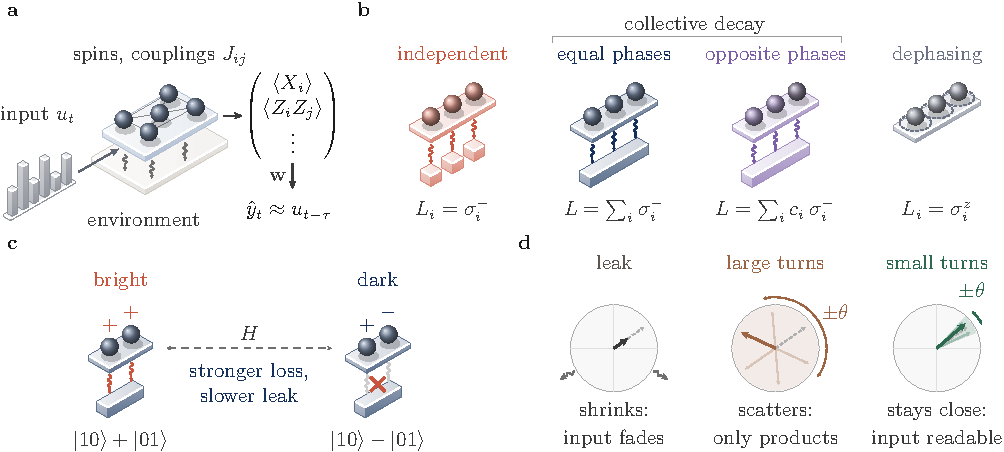
\includegraphics[width=\textwidth]{figures/fig1_concept.pdf}
\caption{\textbf{Engineering how a quantum reservoir leaks.}
\textbf{a}~Inputs drive interacting spins, and a trained linear readout recalls past inputs.
\textbf{b}~Four forms of dissipation with the same total coupling. The darker spins couple with the opposite sign.
\textbf{c}~Two spins on one channel: their decays add (bright) or cancel (dark), and strong loss holds them in the
dark state, the quantum Zeno effect.
\textbf{d}~A stored signal fades because it leaks away or because later inputs turn it at random.}
\label{fig:concept}
\end{figure*}

Processing information over time requires a memory of what came before. A physical system can provide such a memory
because each input changes its state and leaves traces that influence its later response. Reservoir computing uses these
traces to perform a task: an input stream drives a dynamical system, and a weighted sum of quantities describing its
state produces the output. Only these weights are trained; this mapping is called a linear
readout~\cite{Maass2002,JaegerESP2001}. In quantum reservoir computing (QRC), the evolving system is quantum mechanical,
and the readout uses quantities obtained by measuring it~\cite{Fujii2017}. The challenge is to keep earlier inputs
accessible while new information continues to arrive.

The environment shapes how these traces fade. A system can lose energy or information to its surroundings through
processes collectively described as
dissipation~\cite{ChenNurdin2019,Chen2020,Sannia2024,Ricci2026,Domingo2023,Goetting2025,Mujal2023,Franceschetto2026,KobayashiFeedback2024,Cindrak2024,Sannia2026Memory,Paparelle2026}.
Previous work has shown that tuning the dissipation rate improves memory, in some reservoirs with the best performance
at an intermediate loss rate~\cite{Sannia2024,Goetting2025}. Input, interactions, and dissipation can also be optimized
together~\cite{MartinezPenaPRL2021,Baumann2026}. The rate specifies how strongly the environment acts, but the way it
acts is a separate design choice. Engineering this interaction can prepare and protect selected quantum
states~\cite{Poyatos1996,Verstraete2009,Pastawski2011,Harrington2022}. For a system processing an ongoing input stream,
this raises the possibility of controlling which traces of the past survive.

This distinction becomes concrete for a reservoir of interacting spins, each a two-level quantum system. When the spins
decay through separate routes into the environment, they undergo independent decay. When they share a common route, they
undergo collective decay. In certain joint states, the different emission paths interfere and cancel, preventing decay
through that shared route. These protected states are called dark
states~\cite{Dicke1954,AsenjoGarcia2017,Facchinetti2016}. Internal dynamics can still move the system into states that
do decay. If this decay is sufficiently rapid, however, it suppresses those transitions, a phenomenon known as the
dissipative quantum Zeno effect~\cite{FacchiPascazio2002,Zanardi2014,Burgarth2019,Reiter2012}. Stronger loss
therefore slows the escape of information from the protected states (Fig.~\ref{fig:concept}c).

A long-lived state is not yet a usable memory, because each new input changes the same state that stores the past.
A signal that initially depends on one input comes to depend on combinations of several inputs, such as their
product. This mixing is useful for tasks that require relationships between inputs, but it reduces the capacity
available for recalling single inputs~\cite{Dambre2012,Inubushi2017,Cindrak2026}. Reading the memory has a cost as
well, because resolving a weak quantum signal requires repeated preparation and
measurement~\cite{Mujal2023,Cindrak2024,Hu2023}, and a long-lived memory is hard to read if its signal is faint.
Previous work has established memory limits in classical reservoirs~\cite{JaegerESP2001,White2004,Ganguli2008},
explored input strength~\cite{Jaeger2007Leaky}, and investigated how noise and protected states affect quantum
information processing~\cite{Kubota2023,Fry2023,Cheamsawat2025,Akshay2026}. Closest to our work,
Ref.~\cite{Sannia2024} tunes the dissipation rate of the reservoir we study, Ref.~\cite{Cindrak2026} finds one
trade-off between memory and nonlinearity across reservoir schemes, and Ref.~\cite{Akshay2026} reads the output of a
reservoir from a decoherence-free subspace to classify quantum states. The Zeno protection of dark states and the
benefit of a weak input for linear memory are established. How protection, continued input, and measurement together
determine the part of the past that a readout recovers is open.

% Fig. 2 is declared here so that it lands on the top of the third page
\begin{figure*}[!t]
\centering
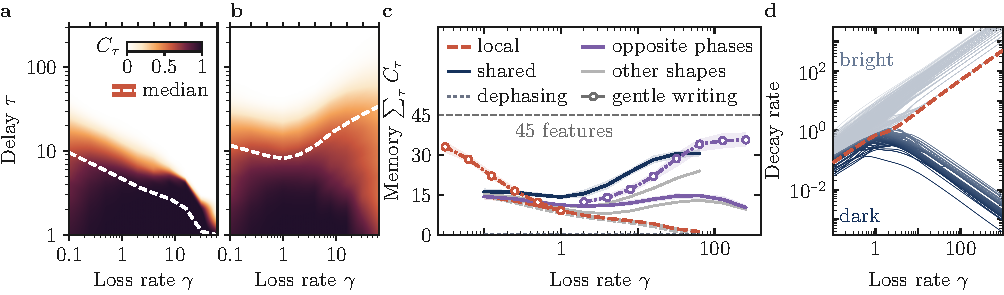
\includegraphics[width=\textwidth]{figures/fig2_clock.pdf}
\caption{\textbf{The decay structure decides whether loss shortens or prolongs the memory.}
\textbf{a,b}~Recall of the input $\tau$ steps back: stronger loss pushes it to shorter delays with independent decay
(a) and to longer delays with the equal-phase channel (b).
\textbf{c}~Linear memory capacity of all channels. Shading marks loss stronger than the couplings
($\gamma>1$).
\textbf{d}~With the equal-phase channel the dark modes decay more slowly as the loss grows, while the slowest mode
of independent decay (dashed) decays faster.}
\label{fig:clock}
\end{figure*}

Here we show that the form of the dissipation sets three properties of a memory (Fig.~\ref{fig:concept}): how long a
stored signal survives, whether and how strongly an input can be written into it, and how strong a signal is left to
measure. First, the decay channel decides at equal total coupling whether stronger loss shortens or prolongs the
memory lifetime. Independent decay shortens it, and collective decay prolongs it through dark states
(Sec.~\ref{sec:clock}). Second, mixing limits how strongly an input can be written. We prove that at a fixed input
amplitude a stored
signal combines on average $s\,t_{\mathrm{mem}}$ inputs, where the mixing fraction $s$ is the part of the stored
signal that one input disturbs and $t_{\mathrm{mem}}$ is the memory lifetime (Sec.~\ref{sec:mixing}). We also prove
that an amplitude that falls as $1/\sqrt{t_{\mathrm{mem}}}$ removes this limit. The share of single inputs then
converges to a value that depends on the input only through its squared amplitude times the lifetime, and this limit
agrees with the five-spin results without a fitted parameter. The phases with which the spins couple to a collective
channel decide whether an input reaches the dark states at all (Sec.~\ref{sec:writing}). Third, the state that the
dissipation leaves behind sets the size of the signal that measurements must resolve. At strong loss a
collective channel whose phases differ from those of the input field recovers the most memory at every measurement
budget, and where the loss can be made weak, independent decay recovers more still (Sec.~\ref{sec:price}).

Together, these results connect the physical survival of information to what a readout recovers from it. The
protection relies on quantum interference, whereas the two theorems hold for every reservoir that meets their
conditions, classical ones included, and give the size of the trade-off between memory and nonlinearity. The form of the
dissipation, the input amplitude and the measurement budget become joint design parameters, and the memory that a
readout recovers becomes a quantity that can be engineered in physical systems that process information over time.

\section{Model}
\label{sec:shapes}
\begin{figure*}[!t]
\centering
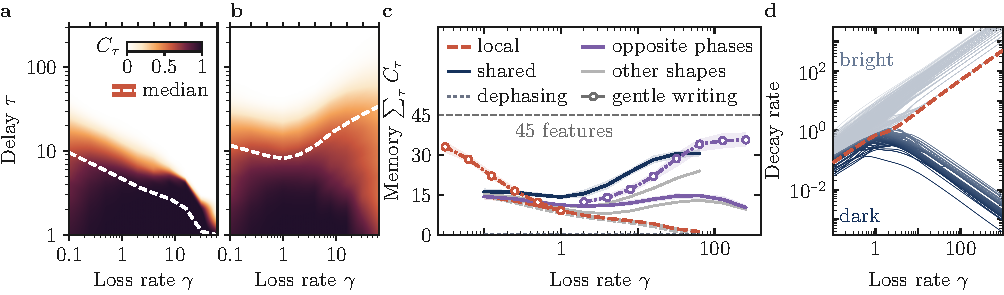
\includegraphics[width=\textwidth]{figures/fig2_clock.pdf}
\caption{\textbf{The decay structure decides whether loss shortens or prolongs the memory.}
\textbf{a,b}~Recall of the input $\tau$ steps back (colour) against the loss rate, for independent decay (a) and the
equal-phase channel (b). The dashed line marks the median delay, which splits the recall in half.
\textbf{c}~Linear memory capacity at the full input strength and with gentle writing, an input that weakens as the
memory lifetime grows (Sec.~\ref{sec:writing}).
\textbf{d}~All decay rates with the equal-phase channel: the dark modes slow down as the loss grows, while the slowest
mode of independent decay (dashed) speeds up.}
\label{fig:clock}
\end{figure*}

The reservoir is the driven spin system of Ref.~\cite{Sannia2024}. Five spins ($N=5$) interact through random
couplings $J_{ij}$, and in each step a random input $u$ between 0 and 1 sets the strength of a transverse field for a
time $\Delta t$:
\begin{equation}
  H(u)=\sum_{i<j}J_{ij}X_iX_j+h\sum_iZ_i+h(1+u)\sum_iX_i ,
  \label{eq:H}
\end{equation}
with Pauli operators $X_i$, $Z_i$ of spin $i$ and a field strength $h$. To weaken the input at a fixed mean drive, we
replace $h(1+u)$ by $h[\tfrac32+\eta(u-\tfrac12)]$, where the amplitude $\eta$ scales how far each input moves the
field. The state $\rho$ of the spins follows a Lindblad master
equation~\cite{Gorini1976,Lindblad1976},
\begin{equation}
  \dot\rho=-i[H(u),\rho]+\sum_k\Bigl(L_k\rho L_k^\dagger-\tfrac12\{L_k^\dagger L_k,\rho\}\Bigr),
  \label{eq:lindblad}
\end{equation}
where the Hamiltonian drives the internal dynamics and each jump operator $L_k$, scaled by one loss rate $\gamma$, is
one way the environment changes the state, such as removing an excitation or erasing a phase.

A linear readout of 45 features, the single-spin and two-spin expectation values, is trained to estimate the input
from $\tau$ steps back. Its recall $C_\tau$, between 0 and 1, is the squared correlation between the estimate and the
input on held-out data. The linear memory capacity $\sum_\tau C_\tau$ adds up the recall over all delays. One unit is
one past input recalled perfectly, and the ceiling is 45, the number of features. The memory lifetime
$t_{\mathrm{mem}}$ says how long the variance of a stored signal survives, and the single-input recall time
$t_{\mathrm f}$ how long one input stays linearly readable on its own (Appendices~\ref{sec:methods-slow} and~\ref{sec:order}). Sections~\ref{sec:clock}
to~\ref{sec:writing} use exact expectation values, as if every measurement were repeated infinitely often, and
Sec.~\ref{sec:price} counts measurements.

We compare decay channels at equal total coupling $\Tr K=\sum_k\Tr L_k^\dagger L_k$ and hold the Hamiltonian fixed
to isolate the effect of the dissipative structure. The generator of Eq.~\eqref{eq:lindblad} has $4^N$ modes,
patterns of change in the state that each decay at their own rate. Equal total coupling fixes their mean rate for
every Hamiltonian, but not the slow modes, which keep a record longest and can become slower or faster
(Appendix~\ref{sec:methods-shapes}). Table~\ref{tab:families} lists the eight channels we studied.

Four of them carry the argument (Fig.~\ref{fig:concept}b). With independent decay every spin loses its excitation on
its own. With collective decay all spins lose it through one shared channel, either with equal phases or with
opposite phases on spins 4 and 5. We call these the equal-phase and the opposite-phase channel. With dephasing every
spin loses its phase. What tells them apart is whether the dissipation leaves only a single stationary state or a
protected subspace that can carry a record. Operators that the dissipation alone leaves unchanged are
protected, although the Hamiltonian can still turn them or couple them to decaying ones. Independent decay protects only
its ground state. Neither collective channel can empty its ten dark states, so every operator on them is protected.
Dephasing keeps the populations, the probabilities of the spin configurations, but erases the coherences between
them. Every step then leaves the fully mixed state, with equal populations and no coherence, unchanged whatever the
input: the dynamics is unital. The driven reservoir relaxes to this state, after which no input leaves a trace, so
dephasing stores nothing.

\section{Results}
\label{sec:results}

\subsection{Dissipative structure controls memory lifetime}
\label{sec:clock}
Increasing the loss separates the channels into distinct memory regimes (Fig.~\ref{fig:clock}). With independent decay, recall retreats to ever shorter delays and the linear memory capacity
falls steadily (Fig.~\ref{fig:clock}a,c). With the equal-phase channel the capacity first dips and then doubles, and
at strong loss inputs fifty steps back are still recalled (Fig.~\ref{fig:clock}b,c). The other channels split the same
way (Fig.~\ref{fig:clock}c, grey): exchange and gain/loss follow independent decay, two collective channels follow the
equal-phase channel, and pairwise decay follows the opposite-phase channel. The decay rates show the split
(Fig.~\ref{fig:clock}d). Without protected operators the slowest rate grows in proportion to $\gamma$ and the memory
lifetime shrinks. With dark states the slow rates fall as $1/\gamma$ and the lifetime grows.

Why does stronger collective decay prolong the memory? In the two-spin picture of Fig.~\ref{fig:concept}c, the dark
state $|{-}\rangle\propto|10\rangle-|01\rangle$ can decay only through the bright state
$|{+}\rangle\propto|10\rangle+|01\rangle$, and the Zeno effect~\cite{Beige2000,FacchiPascazio2002} suppresses this
escape. Its rate falls as $\Omega^2/\gamma$, where $\Omega$ couples $|{+}\rangle$ and $|{-}\rangle$, just as the slow
mode of an overdamped oscillator settles more slowly the stronger the friction.

This protection follows from the strong-loss expansion at fixed system size. At strong loss the reservoir follows its Hamiltonian restricted to the dark
states, which turns the stored state but cannot make it decay. Decay enters only at the next order, when the
Hamiltonian briefly lifts a dark state into a bright one~\cite{Zanardi2014,Reiter2012}. One step is then a rotation
plus a loss that falls as $1/\gamma$ (Eq.~\eqref{eq:reduced}): a nearly orthogonal map with a small but finite decay rate, the
classic recipe for a long memory in a network~\cite{White2004}. Calculations for three to six spins show the same decay out of the dark states, falling as $1/\gamma$ with
different prefactors (Appendix~\ref{app:num-lifetime}).

Two tests show that the dark states hold the memory (Appendix~\ref{app:num-lifetime}). A model of the ten dark states
alone, with no fitted parameter, reproduces the recall of the full reservoir at strong loss. Replacing the protected
components of the state by their time averages after every step, which removes their dependence on the inputs,
destroys all memory beyond a few steps, while the same operation on a randomly rotated set of equal size leaves most
of it. Residual local noise caps this lifetime: for the
equal-phase channel, our estimate requires a ratio of collective to local loss rates that grows quadratically with the
target recall time (Appendix~\ref{app:num-noise}).

Dark states thus protect stored information against decay. With the opposite-phase channel, however, the dark states
are just as protected, yet the capacity returns only to its weak-loss level (Fig.~\ref{fig:clock}c). The reason is
the ongoing input.

\subsection{New inputs mix stored information}
\label{sec:mixing}
Each new input turns the stored state slightly, by an angle that depends on the input (Fig.~\ref{fig:concept}d), so to an old input every newer input acts as noise. Over the
memory lifetime the stored direction takes a random walk of small turns $\pm\theta$ and spreads by about
$\theta\sqrt{t_{\mathrm{mem}}}$. Once the spread reaches about a radian, the record of an old input survives only
multiplied by the inputs that followed it, and a linear readout cannot turn such products back into single inputs.

A stored contribution can therefore depend on one past input or on several jointly. We count the distinct past inputs
that it depends on and call this number $D$. A function of $u_{t-3}$ alone has $D=1$, even if it is nonlinear in
$u_{t-3}$, and $u_{t-3}u_{t-5}$ has $D=2$. The information processing
capacity~\cite{Dambre2012,MartinezPenaIPC2023} also counts how well the readout reconstructs nonlinear functions of
past inputs, and sorting its contributions by $D$ separates information about single inputs from information about
several jointly (Appendix~\ref{sec:order}). The
disturbance caused by one input is measured by its mixing fraction $s$, between 0 and 1: the part of a stored signal
that one input turns differently from the average input. For small turns it grows as the square of the turn. The law
concerns the covariance of the state, how its components fluctuate together across input histories, and assumes that
one pattern of these fluctuations, a single slow direction of the covariance, outlives all others, even when many
slow components of the state share it. Our main theorem then says that a stored contribution
involves on average $s\,t_{\mathrm{mem}}$ inputs, the disturbance per input times the memory lifetime:

\begin{keybox}
\begin{theorem}[Mixing law, made precise in Appendix~\ref{app:law}]\label{thm:law}
Let a reservoir be reset with probability $p$ per step, so that $t_{\mathrm{mem}}\sim1/(2p)$ as $p\to0$, and otherwise turned by
input-dependent unitaries that mix the stored state, leave a single slow direction of the stored covariance, and
write a signal (conditions in Appendix~\ref{app:law}). Pick a stored contribution with probability equal to its share
of the capacity, and let $D$ be the number of distinct inputs it depends on. As $p\to0$, $D/t_{\mathrm{mem}}$ becomes
exponentially distributed with mean $s$, and
\begin{equation*}
  \mathbb ED=s\,t_{\mathrm{mem}}+O(1).
\end{equation*}
\end{theorem}
\end{keybox}
\begin{figure*}[!t]
\centering
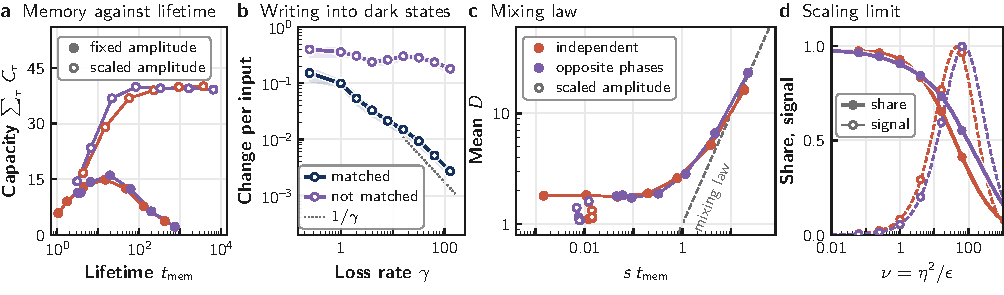
\includegraphics[width=\textwidth]{figures/fig3_price.pdf}
\caption{\textbf{New inputs mix stored information, and gentle writing limits the mixing.}
\textbf{a}~Single-input recall time for four input amplitudes $\eta$, rescaled as the sum of decay and mixing
predicts: for each channel all amplitudes fall on one curve.
\textbf{b}~How strongly one input writes into the dark states of the equal-phase channel: an input aligned with the
channel, the same on every spin, fades as $1/\gamma$, while a pattern that sums to zero over the spins keeps writing.
\textbf{c}~Mean number $D$ of inputs mixed into a stored contribution of the five-spin reservoir, against the mixing
law: at the full input strength it follows $s\,t_{\mathrm{mem}}$, and gentle writing keeps it near one.
\textbf{d}~One qubit, turned by $\theta$ per input and relaxing at the rate $\epsilon$: the stored signal (solid,
relative to its maximum) peaks at an intermediate $\theta^2/\epsilon$, the squared turn accumulated over one relaxation
time (dotted), where single inputs (dashed) still carry 80\% of the capacity.}
\label{fig:mixing}
\end{figure*}


The reason is a race: in each step a fraction $s$ of the stored signal picks up one more input, while a fraction
$1/t_{\mathrm{mem}}$ of it is lost, so the number of inputs follows a geometric distribution, which becomes exponential
for long memories. The same covariance condition extends the law to physical channels without a reset, with the slow decay in place
of the reset (Appendix~\ref{app:physical}), while several slow covariance directions keep distinct mixing scales
(Appendix~\ref{app:slowdir}). Nothing in the law is quantum: classical state-affine reservoirs, whose state is updated
by an input-dependent linear map plus an offset~\cite{GrigoryevaOrtegaSAS2018}, obey it under the same conditions. Dissipation enters through its two factors, the memory lifetime and the disturbance per input.

Exact covariance calculations, Eq.~\eqref{eq:recursion}, support the law in the five-spin reservoir
(Fig.~\ref{fig:mixing}c). At the full input amplitude one input disturbs the stored state only slightly, $s\approx0.02$, and the
mean of $D$ grows with the memory lifetime as $s\,t_{\mathrm{mem}}$ plus an offset of one to two inputs, as
Theorem~\ref{thm:law} allows (Appendix~\ref{app:num-capacity}). At a fixed input strength, a longer memory is
therefore a more mixed one. How must the input strength change with the memory lifetime so that individual
inputs remain readable?

\subsection{Matching input strength to memory lifetime}
\label{sec:writing}
The mixing law suggests weakening each new input as the memory lifetime grows. Because the disturbance $s$ grows as
the square of the turn, keeping $s\,t_{\mathrm{mem}}$ fixed requires an input amplitude proportional to
$1/\sqrt{t_{\mathrm{mem}}}$. We call this gentle writing. A gentler input would write too little: one qubit makes the
trade-off exact (Fig.~\ref{fig:mixing}d, Appendix~\ref{app:qubit}). Its stored signal is largest when the squared turn
per input, accumulated over one relaxation time, is of order one, and only a turn that falls as
$1/\sqrt{t_{\mathrm{mem}}}$ keeps the signal finite as the memory grows.

The single-input recall time shows the same balance. Its rate adds the decay of the stored signal and a mixing rate
that grows as $\eta^2$ (Appendix~\ref{sec:methods-slow}). The decay grows as $\gamma$ with
independent decay and falls as $1/\gamma$ with the opposite-phase channel, so $\eta^2t_{\mathrm f}$ should depend on
loss and input only through $\gamma/\eta^2$ and through $\gamma\eta^2$, respectively. Both collapses hold for four
input amplitudes (Fig.~\ref{fig:mixing}a).

Gentle writing more than doubles the linear memory capacity. In the five-spin reservoir the amplitude falls as
$1/\sqrt\gamma$ for the opposite-phase channel, whose lifetime grows with the loss, and as $\sqrt\gamma$ for independent
decay, whose lifetime grows as the loss weakens (Fig.~\ref{fig:clock}c, circles). With exact readout the capacity rises
from about 15 to 35 units for both channels (Table~\ref{tab:memory}). Since the capacities of all orders add up to the 45
features~\cite{Dambre2012}, the gain moves capacity from combinations of inputs to individual inputs. A
long memory therefore needs no dark states: weak independent decay with gentle writing reaches one too. What dark
states add is a memory that stays long under strong dissipation and grows with the loss.

The phases of the collective channel decide whether an input reaches the protected memory at all. Spin $i$ couples to
the shared channel with the sign $c_i=\pm1$, and the dark states are annihilated by the collective lowering operator
$\sum_ic_i\sigma_i^-$. We call an input field aligned with the channel if its strength on each spin is proportional to
$c_i$. An aligned field $\sum_ic_iX_i$ is the lowering operator plus its adjoint, so it cannot couple two dark states.
It writes into them only through brief excursions into bright states, with a strength that falls as $1/\gamma$, while
the non-aligned part of any other field writes into them directly (Fig.~\ref{fig:mixing}b,
Appendix~\ref{app:num-mixing}). The uniform input of Eq.~\eqref{eq:H} is aligned with the equal-phase channel, so it
writes gently by itself, and this channel comes close to the gain of gentle writing at the full amplitude. With the
opposite-phase channel it is not aligned and must be weakened. This automatic gentle writing relies on exact
alignment: a phase error opens a direct coupling within the dark subspace (Appendix~\ref{app:num-mixing}).

For three spins with the opposite-phase channel we prove both regimes (Appendix~\ref{app:spins}). At a fixed amplitude
single inputs lose their share of the capacity, while with an amplitude $\eta_0/\sqrt\gamma$ they keep it and are
recalled ever further back. The record is written into coherences between the energy levels of the Hamiltonian
restricted to the dark states. Coherence shapes the
performance of spin reservoirs~\cite{Palacios2024}, and erasing these coherences after every input collapses the
stored signal as $1/\gamma^2$. A gentler input, however, writes a fainter record. With exact readout this costs
nothing. With measurements it does.

\subsection{Measurement limits recoverable memory}
\label{sec:price}
Exact expectation values remove the cost of resolving weak signals. A memory whose input strength is matched to its
lifetime grows longer, not larger: it cannot exceed the 45 features, so each delay is recalled more faintly.

For projective readout, each feature is estimated from repeated preparations of the reservoir. Each preparation
replays a finite window of inputs, which grows with the memory lifetime, before it is measured~\cite{Cindrak2024}. We
therefore count the budget in reservoir steps, preparations times replayed steps summed over the measurement settings,
per output step, and simulate the replay (Appendix~\ref{sec:methods-sampling}).

Under this projective-readout protocol, weak independent decay with gentle writing recovers the most memory at a fixed
budget (Fig.~\ref{fig:sampling}a). At a budget of $10^9$ reservoir steps per output step it keeps 34 units, nearly all
of its exact capacity, against 21 for the opposite-phase channel at its best sampled loss rate near $\gamma=64$. The
dark-state memory lasts as long as that of weak independent decay, but its signal is about three times fainter. The
equal-phase channel, whose exact capacity grows with the loss, now loses capacity as the loss grows.

The size of the signal is set by the state that the dissipation leaves behind. An input acts on the stationary state
$\rho_*$ through the commutator with its Hamiltonian, and only the part of this change that lies on the slow modes is
remembered. We call its size the write strength. For this comparison we match the decay-only lifetime $t_{\mathrm{leak}}$, the lifetime with the input held
at its mean value, at 32 input steps (Appendix~\ref{sec:methods-sampling}). There the feature
variance of the seven channels that write follows the write strength over four orders of magnitude
(Fig.~\ref{fig:sampling}b). Collective decay with equal phases, through one channel or two, leaves a polarized state
that the uniform input moves only through bright states, and it stores almost nothing. The opposite-phase channel
leaves a similarly polarized state, but the input is not aligned with this channel and moves it
directly (Sec.~\ref{sec:writing}), so it stores far more. Independent and pairwise decay cool the spins into a state that the
input moves directly, and they store the most. Consistent with earlier work on non-unital damping~\cite{Ricci2026,Domingo2023}, cooling helps here because the input
can move the relaxed state along long-lived modes.

\begin{figure}[!tb]
\centering
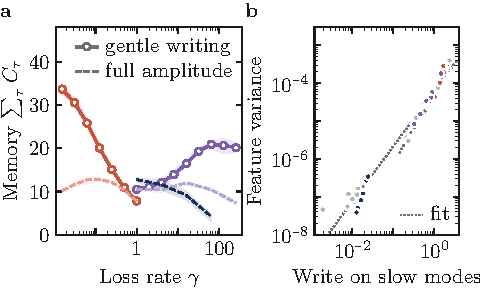
\includegraphics[width=\columnwidth]{figures/fig4_sampling.pdf}
\caption{\textbf{Measurement limits recoverable memory.}
\textbf{a}~Recoverable memory capacity at a budget of $10^9$ reservoir steps per output step: weak independent decay
with gentle writing recovers the most.
\textbf{b}~The signal, the mean variance of the exact features over the inputs, grows with the write strength, how
strongly an input changes the slow modes of the stationary state, for all channels at a matched decay-only lifetime.}
\label{fig:sampling}
\end{figure}

\section{Conclusion}
\label{sec:conclusion}
A useful quantum reservoir must retain a readable record of the past while continuing to accept new information. We
have shown that the structure of dissipation can fundamentally change how this record survives. Independent decay
shortens memory as loss grows, whereas strong collective decay can prolong it by protecting information in dark states
through the quantum Zeno effect. The environment therefore provides a physical means of designing the memory of a
driven quantum system.

Longer storage also leaves more time for subsequent inputs to mix with the stored information. Our mixing law makes this accumulation quantitative. It sets a ceiling on the input strength:
the longer the memory, the more gently new information must be written, so that earlier inputs remain individually
recoverable. In the spin reservoirs studied, weakening the input raises the capacity to recall past inputs from about
15 to 35 units with exact readout, where no input is too weak.

Measurement adds a further requirement: the stored information must produce a signal strong enough to resolve.
Dark-state memories can remain protected for long times while becoming difficult to read. At strong loss a collective
channel with non-aligned phases keeps a readable memory where independent decay keeps none. Where the loss can be made
weak, independent decay recovers the most because its signals are stronger. The resources needed to retrieve information are therefore
part of the design of the memory itself.

Engineering the environment, the input, and the readout together thus provides a route from long-lived quantum
dynamics to memory that a readout can recover. Four rules summarize this design:

\begin{keybox}
\begin{enumerate}[label=(\arabic*),leftmargin=*,itemsep=2pt,topsep=0pt]
\item Collective decay can protect a memory. Stronger loss then makes it last longer, as long as local noise stays
  weak.
\item The input must be able to reach the protected memory. An input aligned with the decay channel hardly writes
  into it.
\item The longer a memory lasts, the more gently each input must be written. Otherwise new inputs mix with the old
  ones.
\item What can be read out depends on how strong a signal the inputs leave, so the measurement budget decides which
  design is best.
\end{enumerate}
\end{keybox}


% Back matter after the conclusion, before the appendices.
\acknowledgments{The authors thank the Quantum Applications and Research Laboratory and the Mobile and
Distributed Systems Group at Ludwig-Maximilians-Universit\"at M\"unchen for institutional support.}

\Needspace{6\baselineskip}
\section*{Data availability}
The code, the data behind every figure, and the derivation and certificates of the three-spin limits are at
\url{https://github.com/eybmits/what-a-dissipative-quantum-system-remembers}.

\Needspace{6\baselineskip}
\section*{Author contributions}
M.B. contributed to conception, methodology, software, analysis, visualization and writing, I.F. and J.W. to
methodology, interpretation and editing, and C.L.-P. and J.S. to supervision and conceptual development. OpenAI Codex
and Claude Code (Anthropic) assisted with manuscript preparation, checks of derivations and references, and simulation,
verification and plotting code. The authors reviewed the outputs and take responsibility for the final content.

\appendix
% Appendix equations are numbered (A1), (A2), ..., restarting in each appendix.
\counterwithin*{equation}{section}
\renewcommand{\theequation}{\thesection\arabic{equation}}
\renewcommand{\theHequation}{\thesection.\arabic{equation}}
\section{Methods}
\label{sec:methods}
This appendix specifies the five-spin simulations and defines the quantities that the main text uses: the reservoir
and its readout, the equal total coupling of the shapes, the slow modes and the strong-loss generator, the order of a
memory and the measurement protocol.

\subsection{Reservoir, readout and memory}
\label{sec:methods-reservoir}
The Hamiltonian of Eq.~\eqref{eq:H} uses $h=1/2$ and couplings $J_{ij}$ drawn uniformly from $[-1,1]$, so the
transverse field runs from $h$ to $2h$. Each input $u$ is drawn uniformly from $[0,1]$ and held for a step of length
$\Delta t=1/2$. We integrate Eq.~\eqref{eq:lindblad} in the 1024-dimensional basis of Pauli operators and evaluate the
step map $E(u)=e^{\Delta t\mathcal L(u)}$ by Chebyshev interpolation in $u$ at ten nodes. Each reservoir draws its
couplings and its input stream from one seed, and every shape uses the same eight seeds, and runs with the input on one spin use the first four. After a washout of
$\max(800,60\gamma)$ steps, at least four times the time to forget, we record the 45 features, the expectation values of $X_i$, $Y_i$, $Z_i$ and of $X_iX_j$,
$Y_iY_j$, $Z_iZ_j$, for 2000 training, 400 validation and 1600 test inputs. The readout is a least-squares fit with an
intercept on the training and validation inputs, and $C_\tau$ is the squared correlation of its estimate with
$u_{t-\tau}$ on the test inputs. The memory sums $C_\tau$ over delays 1 to 300. A delay without any recall reads about
$1/1600$ on the test inputs, so the sum has a floor of about 0.2 units. Figures show the mean of the eight reservoirs,
with bands from the 16th to the 84th percentile.

\subsection{Shapes and equal coupling}
\label{sec:methods-shapes}
Table~\ref{tab:families} lists the jump operators. Their weights give every shape the same total coupling
$\Tr K=N2^{N-1}\gamma=80\gamma$, which fixes the mean decay rate. For a traceless jump $L$ the superoperator trace of its
dissipator is $-2^N\Tr L^\dagger L$, while the commutator with any Hamiltonian is traceless, so the $4^N$ eigenvalues
$\lambda$ of the generator obey
\begin{equation}
  \frac{1}{4^N}\sum\operatorname{Re}\lambda=-\frac{\Tr K}{2^N}
  \label{eq:trace}
\end{equation}
for every shape and every Hamiltonian. The protected operators form the kernel of the dissipator.

\subsection{Slow modes, time to forget and the strong-loss generator}
\label{sec:methods-slow}
The input-averaged step $\bar E=\mathbb E_uE(u)$ is computed by six-point Gauss--Legendre quadrature. Its eigenvalues
$\lambda_j$ give decay rates $\kappa_j=-\ln|\lambda_j|/\Delta t$. If the dissipator protects $n$ operators, the slow
modes are the $n-1$ slowest decaying ones besides the stationary state, and the time to forget is
$t_{\mathrm f}=1/(\Delta t\,\bar\kappa)$, with $\bar\kappa$ their mean rate. Without protected operators we use the
slowest mode. The mean rate adds the leak and the scrambling exactly (Appendix~\ref{app:numerics}). Figure~\ref{fig:clock}d shows instead the decay rates
$-\operatorname{Re}\lambda$ of the generator at the mean input, $u=1/2$. With a shared channel we call the $n-1$
slowest of them dark and all faster ones bright.

Let $\mathcal D$ be the unit-rate dissipator, $\mathcal P=\lim_{t\to\infty}e^{t\mathcal D}$ the projector onto its
kernel and $\mathcal S=(\mathcal D+\mathcal P)^{-1}-\mathcal P$ its inverse on the decaying operators. At strong loss,
eliminating the decaying operators to second order~\cite{Zanardi2014,Reiter2012} gives the generator of the protected
coordinates,
\begin{equation}
  \mathcal G(u)=\mathcal P\mathcal H(u)\mathcal P-\frac1\gamma\,\mathcal P\mathcal H(u)\mathcal S\mathcal H(u)\mathcal P ,
  \label{eq:reduced}
\end{equation}
with $\mathcal H=-i[H,\cdot\,]$. The first term is the Hamiltonian restricted to the protected operators, which turns them, and the second is the leak through brief excursions into bright states.

For gentle writing we replace $h(1+u)$ in Eq.~\eqref{eq:H} by $h[\tfrac32+\eta(u-\tfrac12)]$, which keeps the mean
field: $\eta=\min(1,\gamma^{-1/2})$ for opposite phases and $\eta=\min(1,\gamma^{1/2})$
for local loss.

\subsection{Order of a memory}
\label{sec:order}
A stored signal can depend on one past input or on products of several, and its order counts them: $u_{t-3}$ has
order one, $u_{t-3}u_{t-5}$ order two. Precisely, for independent inputs, every function of the past inputs with finite
variance splits uniquely into orthogonal parts, each of which depends on a fixed finite set of inputs. The order of a part is the size of its set. For signs
$u_t=\pm1$ the parts are the products $\prod_{j\in J}u_{t-j}$, and for continuous inputs one uses orthogonal polynomials
in each input. Quantum channels act affinely on traceless
coordinates~\cite{MartinezPenaOrtega2023,MartinezPenaOrtega2025}, $r_t=A(u_t)r_{t-1}+b(u_t)$. Let $\bar A=\mathbb EA$
be the mean step, $m$ the stationary mean and $\xi=A(u)m+b(u)-m$ the innovation, the change that one input writes,
with covariance $V$. With $\mathcal BX=\bar AX\bar A^{\mathsf T}$, $\mathcal TX=\mathbb E[AXA^{\mathsf T}]$ and
$\mathcal K=\mathcal T-\mathcal B$, the covariance $G_k$ carried by products of order $k$ obeys
\begin{equation}
  G_1=(1-\mathcal B)^{-1}V,\qquad G_{k+1}=(1-\mathcal B)^{-1}\mathcal KG_k .
  \label{eq:recursion}
\end{equation}
The innovation adds the current input alone. The mean step carries a stored product along without adding an input. The fluctuating part $\mathcal K$ of the step multiplies it by the current input, which raises its order by one.
The $G_k$ add up to the stationary covariance $\Sigma$. A readout of features $y=Mr$ explains the share
$\Tr[(M\Sigma M^{\mathsf T})^+MG_kM^{\mathsf T}]$ of order $k$, and these shares add up to the rank of the
readout~\cite{Dambre2012}. For one observable with coordinates $a$ the share of order $k$ is
$a^{\mathsf T}G_ka/a^{\mathsf T}\Sigma a$, and the share of single past inputs is
$a^{\mathsf T}\bar AG_1\bar A^{\mathsf T}a/a^{\mathsf T}\Sigma a$.

The memory time and the mixing fraction come from the slowest mode of the covariance step $\mathcal T$: its eigenvalue
is $1-1/t_{\mathrm{mem}}$, and with its right eigenvector $Q$ and left eigenvector $\ell$ the mixing fraction is
$s=\ell(\mathcal KQ)/\ell(Q)$, as in Appendix~\ref{app:physical}. For five spins we evaluate
Eq.~\eqref{eq:recursion} on the 1023 traceless Pauli coordinates (Appendix~\ref{app:numerics}).

\subsection{Finite sampling}
\label{sec:methods-sampling}
For each step we form the outcome distributions of the three settings and draw $n$ preparations from each. The
readout is fitted as above, with a ridge chosen from fourteen values between 0 and $10^4$ on the validation inputs.
In Sec.~\ref{sec:price} the distributions come from the replay: each output step replays its last $\tau_{90}$ inputs
from $|00000\rangle$, with $n=10^3$ to $10^{8.5}$ in half decades or, for a budget $B$ of preparations times
replayed steps per output step, $n=B/(3\tau_{90})$. Only Fig.~\ref{fig:sampling}b uses the state with the full
history. The matched clock of Fig.~\ref{fig:sampling}b is a leak time
$t_{\mathrm{leak}}=1/(\Delta t\,\bar\kappa_0)$ of 32 steps, where $\bar\kappa_0$ is the mean decay rate of the slow
modes of the generator at the mean input (Appendix~\ref{app:numerics}).

\section{The mixing law}
\label{app:law}
This appendix proves the mixing law of Sec.~\ref{sec:mixing}: in a reservoir that forgets slowly, a stored function
involves on average as many inputs as the mixing fraction of one input times the memory time. The last part extends
the law to physical channels without a reset, which Appendix~\ref{app:spins} needs.

\subsection{Setting and statement}
We describe the reservoir by the $n$ traceless coordinates $r$ of its state in an orthonormal basis of operators, the
Bloch vector for a qubit. A unitary acts on $r$ as a rotation. In each step the reservoir is reset to a fixed state
with a small probability $p$ and is otherwise rotated by $O(u)$:
\begin{equation}
  r_t=(1-p)\,O(u_t)\,r_{t-1}+p\,b .
  \label{eq:reset}
\end{equation}
Here $b$ represents the reset state, and the inputs $u_t$ are independent and identically distributed. A stored
signal loses a fraction $2p$ of its variance per step, so it lasts about $t_{\mathrm{mem}}=1/(2p)$ steps. Three
conditions make the law hold:
\begin{enumerate}[label=(\arabic*),leftmargin=*,itemsep=2pt,topsep=4pt]
\item \emph{The average step forgets.} The average rotation $A=\mathbb EO$ shrinks every vector: its spectral radius
  is below one.
\item \emph{The inputs scramble.} The only covariance matrices that the random rotations leave unchanged on average,
  $\mathbb E[OXO^{\mathsf T}]=X$, are multiples of the identity.
\item \emph{The input writes.} One input changes the state: $\mathbb E\|(O-A)\mu\|^2>0$ with $\mu=(1-A)^{-1}b$.
\end{enumerate}
The first condition means that only products of inputs can be stored for long, the second that a stored signal
spreads evenly over all directions, and the third that there is something to store. The mixing fraction
\begin{equation}
  s=1-\frac{\|A\|_F^2}{n}
  \label{eq:mixing}
\end{equation}
says how strongly one input turns the stored state. For a unit vector $x$ of random orientation,
$\mathbb E\|(O-A)x\|^2=s$: one input turns a fraction $s$ of a stored signal away from the average rotation. The
fraction lies between 0 and 1, and the first condition makes it positive. If the inputs $u=\pm1$ rotate by
$O=e^{u\theta G}$ with a fixed generator $G$, whose eigenvalues are $i\lambda_1,\dots,i\lambda_n$, the average
rotation is $\cosh\theta G$ and $s=\frac1n\sum_j\sin^2\theta\lambda_j$, which grows as $\theta^2$ for small
turns.

\begin{keybox}
\textbf{Mixing law, precise form.} Assume conditions (1)--(3) and take any fixed linear readout. Pick a stored function
with probability equal to its share of the readout's capacity, and let $D$ be its order. As $p\to0$, the ratio
$D/t_{\mathrm{mem}}$ becomes exponentially distributed with mean $s$, and
\[\mathbb ED=s\,t_{\mathrm{mem}}+O(1).\]
Equivalently, products of more than $x\,t_{\mathrm{mem}}$ inputs carry the share $e^{-x/s}$ of the capacity.
\end{keybox}

\subsection{The idea: a race}
A stored signal is spread evenly over all directions. In each step the current input turns a fraction $s$ of it away
from the average rotation, which adds one input to that part, and the reset removes a fraction $1/t_{\mathrm{mem}}$.
On average $1/s$ steps pass before the next input joins a product, and meanwhile it loses a fraction
$1/(s\,t_{\mathrm{mem}})$ of its weight, so products of more than $K$ inputs carry about
\begin{equation*}
  \Bigl(1-\frac{1}{s\,t_{\mathrm{mem}}}\Bigr)^{K}\approx e^{-K/(s\,t_{\mathrm{mem}})} ,
\end{equation*}
an exponential law with mean $s\,t_{\mathrm{mem}}$. The proof makes this bookkeeping exact.

\subsection{Proof}
\label{app:proof}
The proof works with covariance matrices. Appendix~\ref{sec:order} splits the stationary covariance $\Sigma$ of the state into the
parts $G_k$ carried by products of $k$ inputs and gives their recursion, Eq.~\eqref{eq:recursion}: the mean step
$\mathcal B$ carries a stored product along, and the fluctuating part $\mathcal K$ of the step adds one input to it.
In the reset model the mean step is $\mathcal BX=(1-p)^2AXA^{\mathsf T}$, the full step
$\mathcal TX=(1-p)^2\,\mathbb E[OXO^{\mathsf T}]$, and $\mathcal K=\mathcal T-\mathcal B$. We write $\mathcal B_0$,
$\mathcal T_0$ and $\mathcal K_0$ for the same maps at $p=0$.

\paragraph{Step 1: the stored signal is small and spread evenly.}
The stationary mean is $m=p\,[1-(1-p)A]^{-1}b=p\mu+O(p^2)$, so one input writes the change $(1-p)(O-A)m$, of size
$p$. Its covariance $V$ has the trace $p^2v+O(p^3)$ with $v=\mathbb E\|(O-A)\mu\|^2$, which is positive by
condition (3). The random rotations preserve the trace of a covariance and, by condition (2), leave only the identity unchanged. Since they cannot enlarge a covariance, the identity is a simple fixed point with the projector
$X\mapsto(\Tr X/n)\,1$. On every other direction $(1-\mathcal T)^{-1}$ stays bounded as $p\to0$, while on the identity
it equals $1/[1-(1-p)^2]\approx1/(2p)$. The written covariance therefore piles up along the identity:
\begin{equation}
  \Sigma=(1-\mathcal T)^{-1}V=\frac{pv}{2n}\,1+O(p^2).
  \label{eq:slowcov}
\end{equation}

\paragraph{Step 2: few inputs carry almost nothing.}
The mean step forgets by condition (1), so $(1-\mathcal B)^{-1}$ stays bounded as $p\to0$. The recursion then makes
$G_1=(1-\mathcal B)^{-1}V$ of order $p^2$, and the same holds for every $G_k$ with fixed $k$. Measured against
$\Sigma$, which is of order $p$ and has full rank, any fixed set of orders carries a share of order $p$ of the
capacity of any readout, although the shares of all orders add up to its rank. A long memory consists of products of many
inputs.

\paragraph{Step 3: counting the inputs.}
Call $\mathcal F=(1-\mathcal B)^{-1}\mathcal K$ the order transfer, so that $G_{k+1}=\mathcal FG_k$. At $p=0$ it
leaves the identity unchanged, because $\mathcal K_01=1-AA^{\mathsf T}=(1-\mathcal B_0)1$. Its matching left
eigenvector is the weight
\begin{equation}
  \ell(X)=\Tr[(1-A^{\mathsf T}A)X],\qquad \ell(1)=ns ,
  \label{eq:weight}
\end{equation}
since $\ell(\mathcal F_0X)=\Tr\mathcal K_0X=\ell(X)$ when the rotations preserve the trace. For small $p$ the
eigenvalue one moves to
\begin{equation}
  1-\frac{2}{s}\,p+O(p^2):
  \label{eq:ordereig}
\end{equation}
each step up in order costs a fraction $2p/s=1/(s\,t_{\mathrm{mem}})$ of the weight, as in the race. To see this,
differentiate $(1-\mathcal B)\mathcal F=\mathcal K$ at $p=0$ and apply it to the identity, which gives
$(1-\mathcal B_0)\mathcal F_0'1=-2\cdot1$. Its trace is the weight $\ell(\mathcal F_0'1)=-2n$, and dividing by
$\ell(1)=ns$ gives the rate $2/s$.

To turn the eigenvalue into a distribution, weigh order $k$ with $e^{-\lambda pk}$. Summing the recursion gives
$\sum_kz^kG_k=z(1-z\mathcal F)^{-1}G_1$, and as $z=e^{-\lambda p}$ approaches one, only the eigenvalue of
Eq.~\eqref{eq:ordereig} makes the inverse large. With $\ell(G_1)=p^2v+O(p^3)$ and $\beta=2/s$,
\begin{equation}
  \sum_{k\ge1}e^{-\lambda pk}G_k=\frac{pv}{2n}\,\frac{\beta}{\lambda+\beta}\,1+O(p^2).
  \label{eq:laplace}
\end{equation}
Divided by Eq.~\eqref{eq:slowcov}, this is $\beta/(\lambda+\beta)$, the Laplace transform of an exponential
distribution of $pD$ with rate $\beta$. So $D/t_{\mathrm{mem}}=2pD$ is exponential with mean $s$. Because both
covariances are multiples of the identity to leading order, the same holds for the share of the capacity of any
readout. Finally, $\sum_kkG_k=(1-\mathcal F)^{-1}\Sigma=\Sigma/(\beta p)+O(p)$ gives
$\mathbb ED=s\,t_{\mathrm{mem}}+O(1)$.

\paragraph{Two technical points.}
The eigenvalue one of $\mathcal F_0$ is simple: a fixed point of $\mathcal F_0$ satisfies $\mathcal T_0X=X$ and is
therefore a multiple of the identity, and $\ell(1)>0$ rules out a Jordan chain. For $p>0$ every eigenvalue of
$\mathcal F$ lies inside the unit circle, by a Perron--Frobenius argument: $\mathcal F$ maps positive matrices to
positive matrices, and so does $(1-\mathcal F)^{-1}=1+(1-\mathcal T)^{-1}\mathcal K$. The eigenvalues of
$\mathcal F_0$ therefore lie in the closed unit disk, only the simple one equals one, and only the eigenvalue of
Eq.~\eqref{eq:ordereig} makes the sum diverge.

\subsection{When the law needs one slow direction}
Condition (2) matters. Let a classical flag, set by the reset state and never changed, select one of two qubit
rotations about $Z$, by $\pm\pi/6$ or by $\pm\pi/3$, and let the reset state put the flag in either value with
probability $\tfrac12$ and the qubit along $+X$ in both. Each sector obeys the law with its own mixing fraction,
$1/4$ and $3/4$, and a single $Y$ readout sees their mixture, weighted by the variance each sector stores. The
gentler sector stores more, so as $p\to0$ products of more than $x\,t_{\mathrm{mem}}$ inputs carry the share
$w\,e^{-4x}+(1-w)\,e^{-4x/3}$ with $w=0.82$, which exact moments reproduce. One observable then shows two order
scales.

\subsection{Physical channels without a reset}
\label{app:physical}
A physical channel does not reset to a prescribed state, but the proof used the reset only through three facts: one
covariance direction is slow, it leaks at a small rate, and the mean step forgets everything else. The same three
steps therefore prove the law for general channels. Appendix~\ref{app:spins} uses this version, and readers interested in the reset model can skip it.

\emph{Setting.} One step is $r_t=A_u(\epsilon)r_{t-1}+b_u(\epsilon)$ on the coordinates that the inputs can reach,
with a small leak $\epsilon$, and $\mathcal B$, $\mathcal T$ and $\mathcal K$ are formed from $A_u$ as before. We
assume:
\begin{enumerate}[label=(\roman*),leftmargin=*,itemsep=2pt,topsep=4pt]
\item $A_u$ and $b_u$ depend smoothly on $\epsilon$ in mean square, and $b_u$ vanishes at $\epsilon=0$.
\item The mean step forgets at $\epsilon=0$: $\mathbb EA_u(0)$ has spectral radius below one.
\item The channel is mean-square stable for small $\epsilon>0$.
\item One covariance direction is slow: $\mathcal T$ has a simple eigenvalue $1-\kappa\epsilon+O(\epsilon^2)$ with
  $\kappa>0$ and no other eigenvalue near one. At $\epsilon=0$ its right eigenvector is a positive matrix $Q$, and its
  left eigenvector is a weight $\ell$ that is nonnegative on positive matrices, with $\ell(Q)=1$.
\item The input writes along it: the change written by one input, of order $\epsilon$, has covariance
  $\epsilon^2V_*+O(\epsilon^3)$ with $\ell(V_*)>0$.
\end{enumerate}
The reset model is the case $\epsilon=p$, $\kappa=2$, $Q=1$ and $\ell=\Tr/n$. Condition (iv) concerns the
covariance that the random steps carry, not the number of slow modes: at a fixed amplitude the inputs turn the 99
slow dark modes of a shared channel with opposite phases differently in each step and spread a stored signal over
all of them, so that one covariance direction stays slow. With several slow directions, each mixes at its own rate,
as in the example above. Conditions (ii) and (iii) say that the reservoir forgets its starting state on average and in
mean square, (iv) that the random steps spread a stored signal over the slow modes faster than it leaks, and (v) that
the surviving direction is written.

\begin{keybox}
\textbf{Mixing law without a reset.} Under (i)--(v) the mixing fraction $s=\ell(\mathcal K_0Q)$ is positive and at
most one, and $\epsilon D$ becomes exponentially distributed with rate $\kappa/s$. The mean order is
$s/(\kappa\epsilon)+O(1)$: the mixing fraction times the memory time $1/(\kappa\epsilon)$.
\end{keybox}

\emph{Proof.} Steps 1 and 2 carry over. The stationary mean is of order $\epsilon$ by (i) and (ii), and the slow
eigenvalue piles the written covariance up along $Q$,
\begin{equation*}
  \Sigma=\epsilon\,\frac{\ell(V_*)}{\kappa}\,Q+O(\epsilon^2),
\end{equation*}
and every fixed order carries a covariance of order $\epsilon^2$. For the memory of a readout with several features we
also need $Q$ to have full rank on what the readout measures, which holds trivially for one observable. In step 3,
$\mathcal F_0$ has the same fixed points as $\mathcal T_0$, so $Q$ spans them, and $\ell\circ(1-\mathcal B_0)$ is its
left eigenvector, with value $\ell(\mathcal K_0Q)=s$ on $Q$. Differentiating $(1-\mathcal B)\mathcal F=\mathcal K$ at
$\epsilon=0$ and applying it to $Q$ gives $(1-\mathcal B_0)\mathcal F_0'Q=\mathcal T_0'Q$, whose weight
$\ell(\mathcal T_0'Q)=-\kappa$ is the rate of the slow eigenvalue of $\mathcal T$. The order eigenvalue is
therefore $1-(\kappa/s)\epsilon+O(\epsilon^2)$, and the Laplace transform follows as before. It remains to show that $s$ is positive, which also makes the eigenvalue
simple. Because $\mathcal K_0$ maps positive matrices to positive matrices and $\ell$ is nonnegative on them,
$\ell(\mathcal B_0Y)\le\ell(\mathcal T_0Y)=\ell(Y)$ for every positive $Y$, so $0\le\ell(\mathcal
B_0^j\mathcal K_0Q)\le s\le1$ for every $j$. If $s$ vanished, the series $\mathcal F_0=\sum_j\mathcal B_0^j\mathcal
K_0$ would give $\ell(\mathcal F_0Q)=0$, which contradicts $\mathcal F_0Q=Q$ and $\ell(Q)=1$.

\emph{The spin reservoirs.} For three spins the certificates of Appendix~\ref{app:spins} check these conditions. For
five spins we check the law instead of the conditions: Eq.~\eqref{eq:recursion} gives the order distribution exactly,
and it follows the law (below).

\subsection{Numerical check}
Figure~\ref{fig:law} compares the law with exact moments. Beyond the reservoir shown, we tested 24 reservoirs and
readouts in dimensions two to four: two families of three random unitaries, two reset states (a basis state and a
random pure state) and two readouts (all coordinates or one random direction). The largest deviation from the law shrinks in proportion to $p$, from 0.08 at $p=3\%$ to 0.003 at
$p=0.1\%$. The five-spin reservoir follows the law as well (Fig.~\ref{fig:mixing}c): at the largest memories
computed, $s\,t_{\mathrm{mem}}\approx20$, products of more than $K$ inputs carry the share
$e^{-K/(s\,t_{\mathrm{mem}})}$ of the capacity to within 0.14.

\begin{figure}[t]
\centering
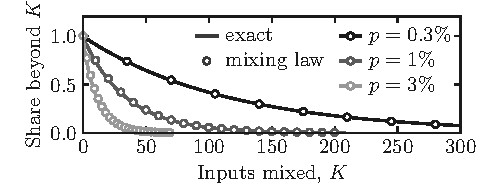
\includegraphics[width=\columnwidth]{figures/figA_law.pdf}
\caption{\textbf{The mixing law.} Share of the capacity carried by products of more than $K$ inputs, for one qubit
that is reset with a small probability $p$ in each step. Lines: exact, circles: the exponential law of
Theorem~\ref{thm:law}.}
\label{fig:law}
\end{figure}

\section{One qubit in closed form}
\label{app:qubit}
This appendix solves the qubit of Sec.~\ref{sec:writing} exactly. At a fixed turn per input the number of inputs
mixed grows as the memory time. A turn that shrinks as the square root of the relaxation rate keeps it finite, and
the stored signal is largest at an intermediate turn.

\paragraph{The model.}
The qubit relaxes towards $+X$ at a rate $\epsilon$, through the jump $\sqrt\epsilon\,|{+x}\rangle\langle{-x}|$, and
the input $u=\pm1$ turns it about $Z$ by $u\theta$ per unit time. Each input lasts one unit of time, and the qubit is
read along $Y$. In the Bloch plane,
\begin{equation}
  \dot x=-\epsilon(x-1)-u\theta y,\qquad \dot y=u\theta x-\tfrac12\epsilon y .
  \label{eq:bloch}
\end{equation}
Over one step this is a linear map of $(x,y)$ plus an offset. For $u=+1$ the map has the form
$\bigl(\begin{smallmatrix}a&-b\\ b&d\end{smallmatrix}\bigr)$ and the offset is $(f,g)$. For $u=-1$ the signs of $b$
and $g$ flip. The input-averaged step is therefore diagonal, the stationary mean lies on the $X$ axis at
$m=f/(1-a)$, and each input writes $u\,v$, with $v=bm+g$, along the measured axis $Y$.

\paragraph{How the orders arise.}
The averaged step keeps the two axes apart, while the input-dependent part swaps them. A signal written into $Y$ must
pass through $X$ and back to pick up more inputs, so $Y$ carries only odd orders. By the
recursion~\eqref{eq:recursion}, covariance passes from $Y$ to $X$ with the factor $b^2/(1-a^2)$ and back with
$b^2/(1-d^2)$. Call the product of the two factors $\chi$. Order $2j+1$ then carries the share $(1-\chi)\chi^j$ of
the capacity of $Y$, and
\begin{equation}
  \mathbb ED=\frac{1+\chi}{1-\chi},\qquad \mathrm{Var}\,Y=\frac{v^2}{(1-d^2)(1-\chi)} .
  \label{eq:qubit}
\end{equation}
Single past inputs carry the share $d^2(1-\chi)$.

\paragraph{Fixed turn.}
Let the relaxation slow down, $\epsilon\to0$, at a fixed angle $\theta$ with $\sin\theta\neq0$. Then
$1-\chi=3\epsilon/\sin^2\theta+O(\epsilon^2)$: the order grows as $1/\epsilon$, $\epsilon D$ becomes exponentially
distributed with rate $3/(2\sin^2\theta)$, and the share of single inputs vanishes, even for exact expectation values.

\paragraph{Gentle writing.}
If instead $\theta^2/\epsilon$ approaches a constant $\nu$, then to first order $a=1-(1+\nu/2)\epsilon$ and
$d=1-(1+\nu)\epsilon/2$, with $b\approx\theta$ and $f\approx\epsilon$, and as $\epsilon\to0$
\begin{equation}
  \begin{aligned}
    \chi&\to\frac{\nu^2}{(\nu+2)(\nu+1)},\\
    \mathrm{Var}\,Y&\to\frac{4\nu}{(\nu+2)(3\nu+2)} .
  \end{aligned}
  \label{eq:qubitlimit}
\end{equation}
The mean order stays finite, and single past inputs keep the share $1-\chi$. Their recall beyond delay $\tau$ is the
fraction $d^{2\tau}$ of the total, so the range that holds 90\% of it grows as $1/\epsilon$:
$\epsilon\tau_{90}\to\ln10/(1+\nu)$.

\paragraph{The best turn.}
The signal of Eq.~\eqref{eq:qubitlimit} is largest at $\nu=2/\sqrt3$ (Fig.~\ref{fig:mixing}d). For $\nu\gg1$ it
vanishes as $4/(3\nu)$, because later inputs scramble earlier ones. For $\nu\ll1$ it vanishes as $\nu$, because each input writes too
little. Among power laws $\theta\propto\epsilon^\alpha$, only $\alpha=1/2$ keeps a finite signal: the turn must fall as
the square root of the relaxation rate, that is, as one over the square root of the memory time. Direct propagation
of the density matrix reproduces all these expressions.

\section{Three spins at strong loss}
\label{app:spins}
\begin{keybox}
\textbf{What we prove.} Take three spins with one shared channel of opposite phases, Eq.~\eqref{eq:H3}, the four
Hamiltonians H1--H4 of Table~\ref{tab:spins}, and every Hamiltonian whose three couplings lie in a small box around
theirs. As $\gamma$ grows:
\begin{itemize}[leftmargin=*,itemsep=2pt,topsep=4pt]
\item At a fixed input amplitude, the order of the memory of $X_1$, divided by $\gamma$, becomes exponentially
  distributed, and the signal in $X_1$ falls as $1/\gamma$ (boxes of half-width 1/32).
\item With the amplitude scaled as $8/\sqrt\gamma$, single past inputs keep a finite share of the capacity of $X_1$,
  and the range of delays that holds 90\% of their recall grows in proportion to $\gamma$ (boxes of half-width 1/512).
\end{itemize}
\end{keybox}

\paragraph{Idea.}
At strong loss, one step of the full master equation is a rotation of the three dark states, up to corrections of
order $\epsilon=1/\gamma$. At a fixed amplitude the two signs of the input rotate the dark states differently. The
stored covariance then has a single slow direction, and the mixing law without a reset applies
(Appendix~\ref{app:physical}). With gentle writing both signs give almost the same rotation. The signal is
written on the scale of the leak and collects in six slow directions, which we follow explicitly. Both arguments end
in finitely many strict inequalities, which a computer checks with rigorous error bounds.

\paragraph{Model and computations.}
The three spins evolve under
\begin{equation}
  H_\eta(u)=\sum_{i<j}J_{ij}X_iX_j+\tfrac12\sum_iZ_i+\tfrac{3+\eta u}{4}\sum_iX_i
  \label{eq:H3}
\end{equation}
with one jump $\sqrt\gamma\,(\sigma_1^--\sigma_2^--\sigma_3^-)$, steps of $\Delta t=1/2$ and signs $u=\pm1$, at
$\eta=1$ (fixed amplitude) or $\eta=8/\sqrt\gamma$ (gentle writing): the field of gentle writing
(Appendix~\ref{sec:methods-slow}) with signs in place of uniform inputs, with the same mean and the same largest change
$\eta/4$. The couplings of the four Hamiltonians H1--H4
are drawn from fixed seeds. For each loss rate we exponentiate the full generator for both signs, solve the
stationary moment equations and evaluate Eq.~\eqref{eq:recursion} for $X_1$ until 99.99\% of its memory is accounted
for. The range $\tau_{90}$ is the smallest delay beyond which less than a tenth of the recall of single inputs
remains.

\paragraph{Both regimes.}
Figure~\ref{fig:spins} shows the two regimes of the box for H3. Gentler writing trades signal for readability, as for
the qubit: at $\eta_0=8$ single inputs keep between
8\% and 81\% of the capacity of $X_1$ for the four Hamiltonians (Table~\ref{tab:spins}), and for H3 this share rises to
67\% at $\eta_0=2$, with a signal 25 times smaller.

\begin{figure}[t]
\centering
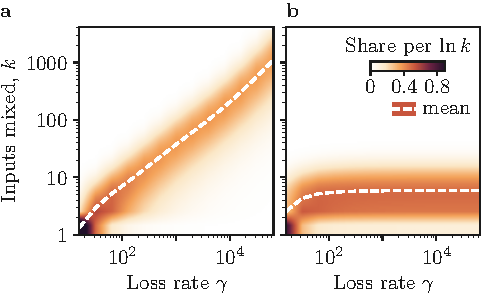
\includegraphics[width=\columnwidth]{figures/figC_spins.pdf}
\caption{\textbf{Three spins, both regimes.} Share of the capacity of $X_1$ carried by products of $k$ inputs
(colour) against the loss rate, for one shared channel with opposite phases (Hamiltonian H3). Dashed: the mean. At a
fixed input strength the number of inputs mixed grows with the loss (a), while with gentle writing it stays small (b).}
\label{fig:spins}
\end{figure}

\begin{table}[t]
\caption{\label{tab:spins}Strong-loss limits for $X_1$ in the four three-spin reservoirs. Fixed amplitude: rate of
the exponential law of the order divided by $\gamma$ (certified). Gentle writing: share of single past inputs and
range of their recall divided by $\gamma$, evaluated at $\gamma=2^{16}$.}
\centering\footnotesize
\begin{tabular}{lccc}
\toprule
 & rate & single-input share & range$/\gamma$\\\midrule
H1 & 78.6 & 0.81 & 0.50\\
H2 & 91.7 & 0.29 & 0.18\\
H3 & 61.4 & 0.08 & 0.24\\
H4 & 132.5 & 0.14 & 0.50\\
\bottomrule
\end{tabular}
\end{table}

\paragraph{One step at strong loss.}
The jump $\sqrt\gamma\,(\sigma_1^--\sigma_2^--\sigma_3^-)$ leaves three dark states: the state with no excitation
and the two single-excitation states with amplitudes $(0,1,-1)/\sqrt2$ and $(2,1,1)/\sqrt6$, which are orthogonal to
the phases of the channel. It empties every other state, so at unit loss rate only the nine operators on the dark
states do not decay. Let $R$ embed these nine coordinates into the full operator space and $R^\flat$ project back
along the decaying operators. Expanding one step in $\epsilon$ gives
\begin{equation}
  E_u=R\,e^{\Delta t\,R^\flat\mathcal H_uR}R^\flat+\epsilon Z_u+O(\epsilon^2),
  \label{eq:slowstep}
\end{equation}
where $\mathcal H_u$ is the commutator with the Hamiltonian of input $u$. The first term rotates the dark states. The
correction $Z_u$ collects the brief excursions into bright states: one at the start of the step, one at its end, and
the leak of Eq.~\eqref{eq:reduced} in between.

\paragraph{Fixed amplitude.}
At $\eta=1$ the dark rotations $O_u$ of the two signs differ, and the computer checks the conditions of the mixing law
without a reset on the eight traceless dark coordinates. The average rotation forgets. The identity is the only covariance that the random rotations leave unchanged. Three constants from the first-order terms of
Eq.~\eqref{eq:slowstep} are positive: the strength with which an input writes, the rate $\kappa$ at which the slow
covariance leaks, and the mixing fraction $s_0=1-\|\mathbb EO_u\|_F^2/8$. The law then gives an exponential
distribution of the order divided by $\gamma$, with rate $\kappa/s_0$ (Table~\ref{tab:spins}), and the variance of
$X_1$ falls as $\epsilon$. A change $r$ of the couplings moves each dark rotation by at most $3r$, which lets the
checks cover the boxes of half-width 1/32.

\paragraph{Gentle writing.}
At $\eta=8\sqrt\epsilon$ both signs give the same leading rotation $E$, generated by the static part of the dark
Hamiltonian. The input enters at order $\sqrt\epsilon$ and the leak at order $\epsilon$. Expanding the step to this order
gives the mean step $E+\epsilon E_1$ and the input-dependent part $u\sqrt\epsilon\,\Delta_1$.

\emph{Where the signal goes.} The rotation $E$ turns each of the three planes of coherence between the dark energy
levels by its own angle, set by an energy gap, and the six phases of these turns differ from each other and from one.
So $E$ leaves only the populations unchanged, and on them $E_1$ generates a slow population dynamics with a unique stationary state
$m_*$. An input therefore writes $\pm\sqrt\epsilon\,v$ with $v=\Delta_1m_*$, which lies in the coherence planes: a new
input first turns a population into a coherence.

\emph{Six slow directions.} The covariances that $E$ leaves unchanged form a six-dimensional space: the three
covariances of the two population coordinates and one isotropic covariance in each coherence plane. Over $1/\epsilon$
steps a covariance in this space changes under two generators, both certified stable. $K_B$ describes how the mean
step lets a stored signal decay, and $K_T$ adds the random signs of later inputs, which turn a stored signal into
products. With $P_6$ the projection onto the six directions, the single-input part of the stored covariance and the
full covariance approach $W_*=-K_B^{-1}P_6(vv^{\mathsf T})$ and $\Sigma_*=-K_T^{-1}P_6(vv^{\mathsf T})$.

\emph{Limits.} With $a$ the coordinates of $X_1$, the share of single past inputs in the memory of $X_1$ tends to
$a^{\mathsf T}W_*a/a^{\mathsf T}\Sigma_*a$. After $t/\epsilon$ steps the remaining single-input recall is the fraction
$a^{\mathsf T}e^{tK_B}W_*a/a^{\mathsf T}W_*a$, which crosses 0.1 once, and the crossing is the range divided by $\gamma$.
The certificates show $a^{\mathsf T}W_*a>0$, and since $\Sigma_*\succeq W_*$ the share is positive. In the boxes of
half-width 1/512 the six angles stay separated and both generators stay stable, so the limits stay positive.

\paragraph{Why coherence carries the memory.}
Returning bright population to the dark subspace after every step leaves the leading terms of the scaled step
unchanged, so it keeps the same limits. Dephasing in the dark energy basis, by contrast, removes the coherence planes
into which $v$ writes. Restricted to populations, the two signs then differ only at order $\epsilon^{3/2}$, because the
response of a population at order $\sqrt\epsilon$ is a coherence, while the populations still follow the slow
population dynamics. A new input thus writes a vector of size $\epsilon^{3/2}$, the slow dynamics sum its square over
$1/\epsilon$ steps, and the stored signal is of order $\epsilon^2$: the collapse as $1/\gamma^2$ of
Sec.~\ref{sec:writing}. Numerically, applying the loss-only projector $\mathcal P$ after every step, with or without
dephasing in the energy basis of the projected Hamiltonian, the variance of $X_1$ stays between $10^{-4}$ and
$2\times10^{-3}$ from $\gamma=2^8$ to $2^{18}$ when the coherences are kept and falls as $\gamma^{-2}$, by six orders
of magnitude, when they are erased. At a fixed input amplitude it falls as $1/\gamma$.

\paragraph{What the computer checks.}
The attached archive \texttt{spin\_certificates.zip} contains the generators, the exact couplings and the interval
programs. They enclose every quantity above in intervals with rigorous rounding (ball arithmetic of Arb, python-flint
0.9.0) and check each strict inequality of this appendix at 256 bits, and at 192 bits they reproduce the archived
enclosures. A second program, sharing no routine with
them, builds the full finite-rate maps and extrapolates to infinite loss. It agrees with
the certified rates and limiting recalls to better than one part in a million.

\section{Numerical details and supporting checks}
\label{app:numerics}
This appendix backs the main text: each paragraph names the section it supports, says what we checked and gives what
is needed to reproduce it.

\paragraph{Recall and memory (Sec.~\ref{sec:clock}).}
Figures smooth recall curves for display only: each delay is averaged with its neighbours, with weights that fall
linearly to zero at a fifth of the delay, and no sum uses the smoothed values. The maps of Fig.~\ref{fig:clock}a,b are
computed at $\gamma=0.1$, 0.25 and $2^{-1}$ to $2^6$ in powers of two and interpolated by shifting each recall profile
along the delay. Figure~\ref{fig:clock}c stops one and two shared channels at $\gamma=64$, where their recall at the
full amplitude starts to reach past the 300 delays we sum. Summed over all delays with exact moments
(Appendix~\ref{sec:order}), their memory keeps rising up to $\gamma=256$. With gentle writing, delays beyond 300 add
about 1\% to the memory of opposite phases.

\paragraph{Dark states (Sec.~\ref{sec:clock}).}
Both tests act on the 100 dark coordinates. For the dark-state model we write $\mathcal P=RR^\flat$ with $R^\flat R=1$,
where $R$ embeds the dark coordinates $\alpha$, evolve $\alpha$ under Eq.~\eqref{eq:reduced} and record the same 45
features of the full state $(R-\mathcal S\mathcal H(u)R/\gamma)\,\alpha$. The readout is trained on them exactly as for
the full reservoir, and the model has no fitted parameter (Fig.~\ref{fig:darkmodel}a). For the erasure test we replace
the dark coordinates after every step by their time average, $r\mapsto r-RR^\flat(r-\bar r)$. The control erases the
dark subspace rotated by a random product of single-spin unitaries. Recall is measured at delays 1 to 100 with 800
training, 200 validation and 800 test inputs (Fig.~\ref{fig:darkmodel}b).

The leak out of the dark states falls exactly as $1/\gamma$: for one shared channel $\gamma\bar\kappa$ approaches
$\kappa_{\mathrm c}=2.945$ from $\gamma=512$ on, so $t_{\mathrm f}$ grows in proportion to $\gamma$, while it levels off
near 56 steps with opposite phases and near 110 with pairwise loss. The second-order calculation of
Eq.~\eqref{eq:reduced} gives the same $\kappa_{\mathrm c}$ at five spins and 1.4, 2.1 and 3.4 at three, four and six
spins: the size of the reservoir sets only the strength of the leak.

\begin{figure}[t]
\centering
\includegraphics[width=\columnwidth]{figures/figD_dark.pdf}
\caption{\textbf{Dark states hold the memory.} One shared channel.
\textbf{a}~The dark states alone (circles), with no fitted parameter, reproduce the recall of the full reservoir
(lines).
\textbf{b}~Erasing the dark states after every step destroys the memory, while erasing a rotated copy of the same size
leaves most of it (dark line: intact reservoir, $\gamma=16$).}
\label{fig:darkmodel}
\end{figure}

\paragraph{Time to forget and phases (Sec.~\ref{sec:mixing}).}
We compute $t_{\mathrm f}$ at $\eta=1$, $\tfrac12$, $\tfrac14$ and $\tfrac18$, for $\gamma$ from $2^{-8}$ to $2^6$ with
local loss and from $2^{-2}$ to $2^{12}$ with opposite phases. The collapses of Fig.~\ref{fig:mixing}a do not depend on
how the time to forget is defined: with the slowest mode in place of the mean rate they hold to within 11\% wherever
forgetting takes more than four steps, and they hold as well with the input on one spin. Weakening the input moves the
best loss rate: on one reservoir with exact moments, the memory peak of local loss moves from $\gamma\approx1/16$ at
$\eta=1$ to $1/64$ at $\eta=\tfrac18$, and the best memory rises from 16 to 39 units.

The write per input of Fig.~\ref{fig:mixing}b is $2\|R^\flat[E(\tfrac34)-E(\tfrac14)]r_*\|$ at the stationary state
$r_*$ of the equal-phase channel, for the input patterns $(1,\dots,1)$ and $\sqrt2\cos(2\pi i/5)$ multiplying $X_i$.
Along the phases it falls as $1/\gamma$, to 0.003 at $\gamma=128$, while across them it falls only slowly, to 0.18. Opposite
phases are the equal-phase channel with the field on spins 4 and 5 reversed, up to a relabelling of the random
couplings (a turn of these spins by $\pi$ about $Z$).

\paragraph{Orders and capacities (Secs.~\ref{sec:mixing} and~\ref{sec:writing}).}
The order distribution of Eq.~\eqref{eq:recursion} uses six-point Gauss--Legendre quadrature for the expectations over
the input and solves the equations $X-\bar AX\bar A^{\mathsf T}=C$ in the eigenbasis of $\bar A$. The shares of the 45 features are summed until the rest falls below $10^{-8}$, or until successive orders shrink at a settled ratio, whose
geometric tail we add. The linear recall follows from the same moments,
$C_\tau=c_\tau^{\mathsf T}\Sigma_y^{-1}c_\tau/\mathrm{Var}\,u$ with $c_\tau$ the covariance of the features with
$u_{t-\tau}$ and $\Sigma_y$ their covariance, and reproduces the simulated memories to a median of 2\%. Three steps of
inverse iteration on $\mathcal T$, from the input's covariance $V$ and from the identity, give $t_{\mathrm{mem}}$, $Q$
and $\ell$. Loss rates run in powers of four over the ranges of Fig.~\ref{fig:mixing}c, and with gentle writing to
16384 and $1/4096$, on four reservoirs, two at the largest memory times. With local loss the mean order follows the law
as well, within 2.2 of $s\,t_{\mathrm{mem}}$ up to $s\,t_{\mathrm{mem}}=18$.

\paragraph{Measurement (Sec.~\ref{sec:price}).}
We measure the signal by the variance of a feature over the test inputs, averaged over the features. Gentle writing
makes it fainter: with opposite phases it falls from $8\times10^{-5}$ at the full amplitude to $5\times10^{-6}$, against
$7\times10^{-5}$ with local loss and gentle writing at $\gamma=1/32$. Restarting each run from $|00000\rangle$, as the
replay does, raises these to $4\times10^{-5}$ and $1.2\times10^{-4}$. At the full amplitude the signal of the
equal-phase channel falls from $2\times10^{-4}$ at $\gamma=1$ to $4\times10^{-7}$ at $\gamma=64$, which is why this
channel loses memory as the loss grows once measurements are counted.

The replayed range $\tau_{90}$ grows with the clock, though more slowly: along the gentle line of opposite phases from
about 30 steps at $\gamma=16$ to 130 at $\gamma=256$. The budget sets the best loss rate: at $10^{10}$ preparations
times replayed steps the optimum of the equal-phase channel moves from $\gamma=1$ to about 16, with 17 units, while
opposite phases with gentle writing peak near $\gamma=64$ with 25. Below the crossings the full amplitude wins: at
$10^4$ preparations it keeps 11 units with local loss and 8 with opposite phases, against 9 and 3 with gentle writing.
With the input on one spin, which writes more gently by itself, the crossings move to about $3\times10^5$ and
$4\times10^6$ preparations. With the full history, eight times more training inputs change the sampled memory by less
than 1.3 units.

For the matched clock of Fig.~\ref{fig:sampling}b we find, for every shape and reservoir, the loss rate at which
$t_{\mathrm{leak}}=32$ steps, at weak loss without protected operators and at strong loss with them, and run the
reservoir there with $\eta=\sqrt{4/32}$. The write is $-i[H_{\mathrm{in}},\rho_*]$ with $H_{\mathrm{in}}=h\sum_iX_i$ and
$\rho_*$ the stationary state, projected spectrally onto the slow modes: the protected ones, or without protected
operators those decaying at most four times faster than the slowest. The memory that survives $10^6$ preparations
rises with the write, from 0.3 units for the shared channels to 17 for local loss, and power laws fitted within the
shapes without and with dark states (dotted in Fig.~\ref{fig:sampling}b) have exponents 2.0, as linear accumulation of
the write predicts, and 1.5.

\paragraph{Ordinary noise (Sec.~\ref{sec:conclusion}).}
Adding local loss $\sqrt{\gamma_{\mathrm{loc}}}\,\sigma_i^-$ to a shared channel gives
$\bar\kappa=\kappa_{\mathrm c}/\gamma+\kappa_{\mathrm l}\gamma_{\mathrm{loc}}$, where to first order $\kappa_{\mathrm l}$
is the trace of the added dissipator on the 99 slow dark modes divided by 99, $140/99\approx1.414$. Local dephasing
$\sqrt{\gamma_\phi}\,Z_i$ adds $\kappa_\phi\gamma_\phi$ with $\kappa_\phi=403.2/99\approx4.073$, and the full spectra
reproduce both coefficients to within 0.2\%. A time to forget of at least $T$ steps,
$\kappa_{\mathrm c}/\gamma+\kappa_{\mathrm l}\gamma_{\mathrm{loc}}\le1/(\Delta t\,T)$, then needs
$\gamma/\gamma_{\mathrm{loc}}\ge4\kappa_{\mathrm c}\kappa_{\mathrm l}\,\Delta t^2T^2\approx4.2\,T^2$, or $12\,T^2$ for
dephasing.


\begingroup
% the reference list is set one size smaller than the text, without font expansion
\small\microtypesetup{expansion=false}
\bibliographystyle{quantum}
\bibliography{references}
\endgroup

\end{document}
